{\textbf{实现控制单元(CU)的方式有两类}}(2009年第19题已经考过):

\textbf{1)组合逻辑控制(或称为硬布线逻辑控制):}由基本的门电路组合实现。这种方式实现的控制器的处理速度快,但电路庞杂,制造周期长,不灵活,可维护性差。

\textbf{2)微程序控制:}仿照程序设计的方法编制每个机器指令对应的微程序,每个微程序由若干条微指令构成,各微指令包含若干条微命令。所有指令对应的微程序放在只读存储器中。当执行到某条指令时,取出对应微程序中的各条微指令,译码产生对应的微命令,送到机器相应的地方,控制其动作。

{\textbf{1.微指令的基本格式}}

微指令的基本格式如下图所示,共分两个字段,一个为操作控制字段,该字段发出各种控制信号;另一个为顺序控制字段,该字段可指出下条微指令的地址(简称下地址),以控制微指令序列的执行,这个其实类似于PC。

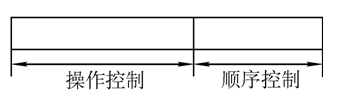
\includegraphics[width=2.08333in,height=0.58333in]{png-jpeg-pics/D02093D34A87FA443383A3FA46BE796B.png}

{\textbf{2.微指令的编码方式}}

微指令的编码方式又称为微指令的控制方式。它是指如何对微指令的控制字段进行编码,以形成控制信号。

\textbf{1)直接编码(直接控制)方式。}在微指令的微命令字段中每一位都代表一个微命令。设计微指令时,选用或不选用某个微命令,只要将表示该微命令的对应位设置成1或0就可以了。因此,微命令的产生不需要译码,如下图所示。

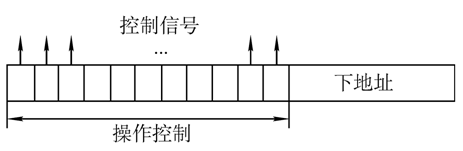
\includegraphics[width=3.01042in,height=0.97917in]{png-jpeg-pics/38B2985EEE6550D6DC4F8E528D13FE8A.png}

\textbf{2)字段直接编码方式。}将微指令的微命令字段分成若干小字段,把互斥性微命令(在同一微指令周期中不能同时出现的微命令称为互斥性微命令)组合在同一字段中,把相容性微命令组合在不同的字段中。每个字段独立编码,每种编码代表一个微命令且各字段编码含义单独定义,与其他字段无关,这就是字段直接编码方式,如下图所示。

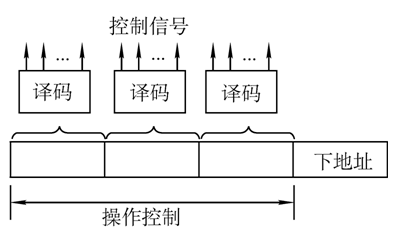
\includegraphics[width=3.11458in,height=1.78125in]{png-jpeg-pics/79B04EA02F4B63DE41B929D9BCDA782E.png}

\textbf{3)字段间接编码方式。}一个字段的某些微命令需由另一个字段中的某些微命令来解释,由于不是靠字段直接译码发出的微命令,故称为字段间接编码,又称隐式编码。这种方式可进一步缩短微指令字长,但因削弱了微指令的并行控制能力,因此通常作为字段直接编码方式的一种辅助手段。

\textbf{4)混合编码方式。}混合编码方式由直接编码与字段(直接或间接)编码混合使用。

{\textbf{3.微指令序列地址的形成}}

{后续微指令的地址主要考查两种形成方式。}

\textbf{第一方式:}后续微指令的地址可以由微指令的下地址字段直接给出,这种方式又称为断定方式(2014年统考真题已经考查)。

\textbf{第二方式:}后续微指令的地址还可以根据机器指令的操作码形成。微地址形成部件实际是一个编码器,其输入为指令操作码。即将机器指令的操作码送入地址译码器进行译码,输出结果就是对应该机器指令微程序的首地址。然后拿着首地址去微命令寄存器找到相应的微命令。

{\textbf{4.微指令格式}}

微指令格式与微指令的编码方式有关,其通常分为\textbf{水平型微指令和垂直型微指令}两种。水平型微指令与垂直型微指令的比较见下表。

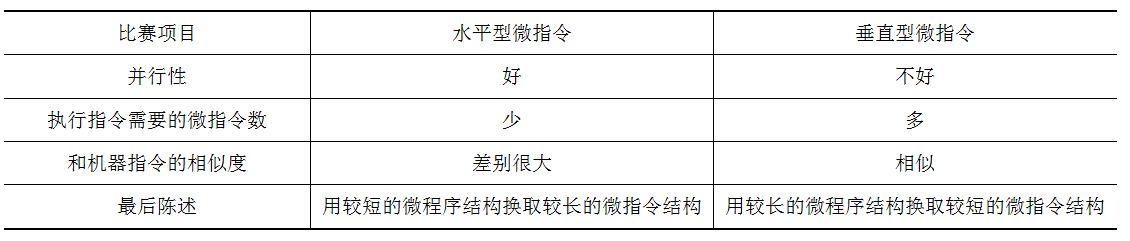
\includegraphics[width=3.12500in,height=0.66667in]{png-jpeg-pics/F153F990ACA74EB73925D3D13D61CDF4.png}

{\textbf{5.微操作的节拍和安排设计步骤}}

每一条机器指令要完成的操作是固定的,因此不论是组合逻辑设计还是微程序设计,对应相同的CPU结构,两种控制单元的微操作命令和节拍安排是极其相似的。\textbf{微程序控制单元在取指周期发出的微操作命令及节拍安排如下:}

T0 (PC)→MAR,1→R\\
T1 ~M(MAR)→MDR,(PC)+1→PC\\
T2 (MDR)→IR,OP(IR)→微地址形成部件
